\chapter{1. Introduction}

\begin{quote}
\textit{Around the world, people are experiencing adverse health effects as a result of poor air quality.  It is currently impossible for them to accurately track and understand their exposure using affordably-priced technology.  While consumer monitoring solutions claim to address this disparity, time and again they are shown to be unreliable. \newline 	What if we could make cheap, personal air quality data trustworthy?  What could individuals, communities, and research organizations achieve with this new data?  How could we facilitate an open and collaborative ecosystem for sharing this data?} 
\newline
\end{quote}

In 2014, the World Health Organization (WHO) revised previous estimates of air pollution related mortality-- more than doubling them. \cite{who2014} Shockingly, it is now estimated that one in eight total global deaths are the result of air pollution exposure, making air pollution the world's single largest environmental health risk. \cite{who2014, who2014_2}  These revisions hint at the complexity of monitoring air pollution-- the link from standard measurement techniques to personal exposure, and the further link from exposure to health, are still difficult to model.  Failure to understand these relationships can undermine and obfuscate the health risks facing the global community. \cite{who2014, who2014_2, filley1954, allred1989, schwartz2005}

For the millions of people living in toxically polluted cities around the world, understanding their daily pollution exposure-- and making informed changes to minimize it-- could literally lengthen their lives.  Affordable consumer devices have exploded over the last several years to address this need; however, none have proven reliable under real-world conditions. \cite{williams2014}  Research continues to drive smaller and cheaper sensor technology, but the underlying physics and their associated manufacturing costs limit what is currently feasible.

The lack of reliable personal monitoring solutions is also a systemic problem.  In many cities, political rhetoric and policy are in play as citizen groups and research organizations mobilize around the issue.  Local governments are installing distributed air quality networks-- in some cases with citizen groups at the helm.  Unfortunately, pervasive misinformation about the data quality of these new networks makes it easy for smart city initiatives to find themselves with solutions that yield limited benefits.  At best this is a waste of time and money; at worst, it may precipitate unnecessary panic or ill-informed policy-making.  

Proper education of politicians, citizen sensing groups, and the public is an important and difficult undertaking.  In many cases, air quality rhetoric has out-paced its understanding, and the advocates working to correctly frame the discussion are playing from behind.  Long-term, a market saturated with unreliable instruments could lead to disillusionment with the technology and friction surrounding the issue and its proponents.

While well-intentioned organizations figure out how to interact and guide community sensing initiatives to act correctly and responsibly, they also have a lot to gain from distributed, reliably-measured personal data.  A breakthrough in personal sensing could unlock amazing insight into pollution modeling and epidemiology.  Unfortunately, there are open questions in the environmental sensing world about how to store, interact with, characterize, and use these data.  Even simple sharing of data amongst well informed organizations and researchers-- without the confounding factor of unknown data quality-- is an actively-debated issue.  Differences in data labeling and data collection methodology make it difficult to agree upon a set of definitions and standards.

As we've seen, there are many serious challenges and much unrealized potential-- for individuals, policy-makers, and organizations-- that arise from the lack of trustworthy, affordable air quality monitoring approaches.  Many researchers attempt to solve this problem directly by designing smaller and cheaper sensor technologies.  Unfortunately, it is incredibly hard to improve the cost/reliability of a mature technology by simply re-optimizing the same core operating principles.  Critically, there is also no agreed-upon standard for characterizing these device in real-world conditions.    Many consumer devices unwittingly find themselves re-hashing the same core design principles and claiming improvement based on unrealistic, controlled laboratory tests.   

In this thesis, we explore a novel approach to advancing the quality of affordable, personal air quality data.  Instead of fighting to \textit{make} more reliable distributed sensors, our goal is to \textit{predict} when a sensor is accurate and when it is not.  

An affordable sensor may lose accuracy in predictable ways.  An otherwise poor quality sensor may provide very trustworthy, repeatable data for a narrow set of climates, geographies, or seasons.  Previously, there has been no systematic way to understand, classify, or predict these patterns.  With this work, we test the limits of this approach and build a device that takes advantage of it.  The learnAir system doesn't attempt to be more accurate than similar cost systems.  It simply predicts when it is likely to be accurate, and when it is likely not to be.  

The ramifications of such a design are numerous. If it succeeds, it will provide more accurate personal exposure information than comparable sensor systems-- empowering individuals to more intelligently address any health concerns.  It will also empower researchers and organizations to interact with data from historically untrustworthy sources.  Furthermore, the algorithms underlying the learnAir system might be useful in matching existing sensors with climates and geographies where they will succeed-- not only informing and improving the decision-making behind large-scale installations, but fundamentally altering the conversation to reflect its true complexity.  

The learnAir system is designed in a scalable way, with an easy-to-use, open backend.  The structure allows sensors to compare themselves against one another, learn from one another, and automatically improve their learning models over time.  As more sensors are added to the network, each benefits from the collective, shared data.  For instance a sensor tested and deployed in the California summer will learn from the same type of sensor tested in a Boston winter-- forming a more accurate and complete real-world model than either in isolation.  This novel backend design has powerful implications for the air quality community.  It not only points to principles for sharing air quality data, but also stakes a claim in how researchers and engineers may utilize any distributed data set where quality is a significant variable.
 
The learnAir hardware is a portable, Bluetooth Low Energy (BLE) connected system that talks to its database through a smartphone app.  In the cloud, its data is automatically compared to any nearby, higher quality EPA reference sensors, and the device learns to predict its own accuracy based on this comparison.  LearnAir uses weather data, as well as on-board sensors that measure temperature, humidity, light, wind, motion, and other pollutants, to predict its accuracy.  

In other words, when the device is next to a higher quality sensor, it will automatically compare itself against the reference to see when its readings are consistent.  If it discerns an inconsistent reading, it analyzes the weather and other ambient conditions to gauge whether there are any patterns that correlate with its inaccuracy.  It also analyzes patterns that would suggest it is accurate.

Thus, every measurement learnAir makes comes with a prediction as to whether it is correct (as compared with a reference measurement method), as well as a probability that it has guessed its correctness accurately.  This information is based on a shared data resource, which houses a constantly updating sensor model.  This model takes into account all of the measurements ever reported to the system by that type of sensor.   

In order to build this device and the supporting infrastructure, and in order to validate that a system of this type is useful, we pose the following preliminary questions:  

\enlargethispage{10\baselineskip}

(1) How well can machine learning algorithms predict the accuracy of an unreliable sensor if some information is available about the sensor's environment?  What is the best approach to applying machine learning to this problem?  Answering this question successfully has implications beyond air quality sensor networks, informing new topologies for high/low quality sensor interaction and system design for a range of networked systems.

(2) How can different systems of variable quality be supported using an intelligent, scalable, and open data structure?  In this thesis we create many new tools for crawling and interacting with distributed data.  The implications of this work again reach beyond air quality, in fields ranging from large-scale data sharing to the Internet of Things.

This thesis (1) answers the two foundational questions outlined above, and (2) uses the results to build a novel, deployable system.  In it, we test whether machine learning can provide a more nuanced understanding of when and how inexpensive sensors succeed, to elevate their trustworthiness.  We build a scalable database that supports scalable learning algorithms, where sensor data of any quality can co-exist seamlessly.  Finally, we demonstrate a system that takes advantages of these techniques, evokes a fruitful dialog in the citizen sensing community, and puts that technology in the palm of your hand.


%Currently, the EPA validates cheap sensors with a labor-intensive co-location process, where consumer devices are placed next to a high quality FRM (Federal Reference Measure) sensor and compared over several months/seasons.  Measurements are then collected and analyzed by hand, resulting in a simple 'yes/no' answer regarding whether or not the sensor is useful based on it's overall agreement with the reference standard.  

%fog, humidity, near road, traffic, wind for optical
%temp, humidity, cross-sensitivity, near road for cross-sensitivity, traffic

%here's text referencing the (Table \ref{tab:sample_table}).
%
%\begin{table}
%  \centering
%  \begin{tabular}{l l l l l}
%    Column A & Column B & Column C & Column D & Column E \\
%    \toprule
%    A & B & C & D & E
%  \end{tabular}
%  \caption{A meaningless table}
%  \label{tab:sample_table}
%\end{table}

%Here's text referencing the margin figure (Figure \ref{fig:spin_margin}).
%
%\marginnote{\textbf{Margin Note:} Check it out, here's a margin note.}
%
%\begin{marginfigure}[{-10cm}]
% 	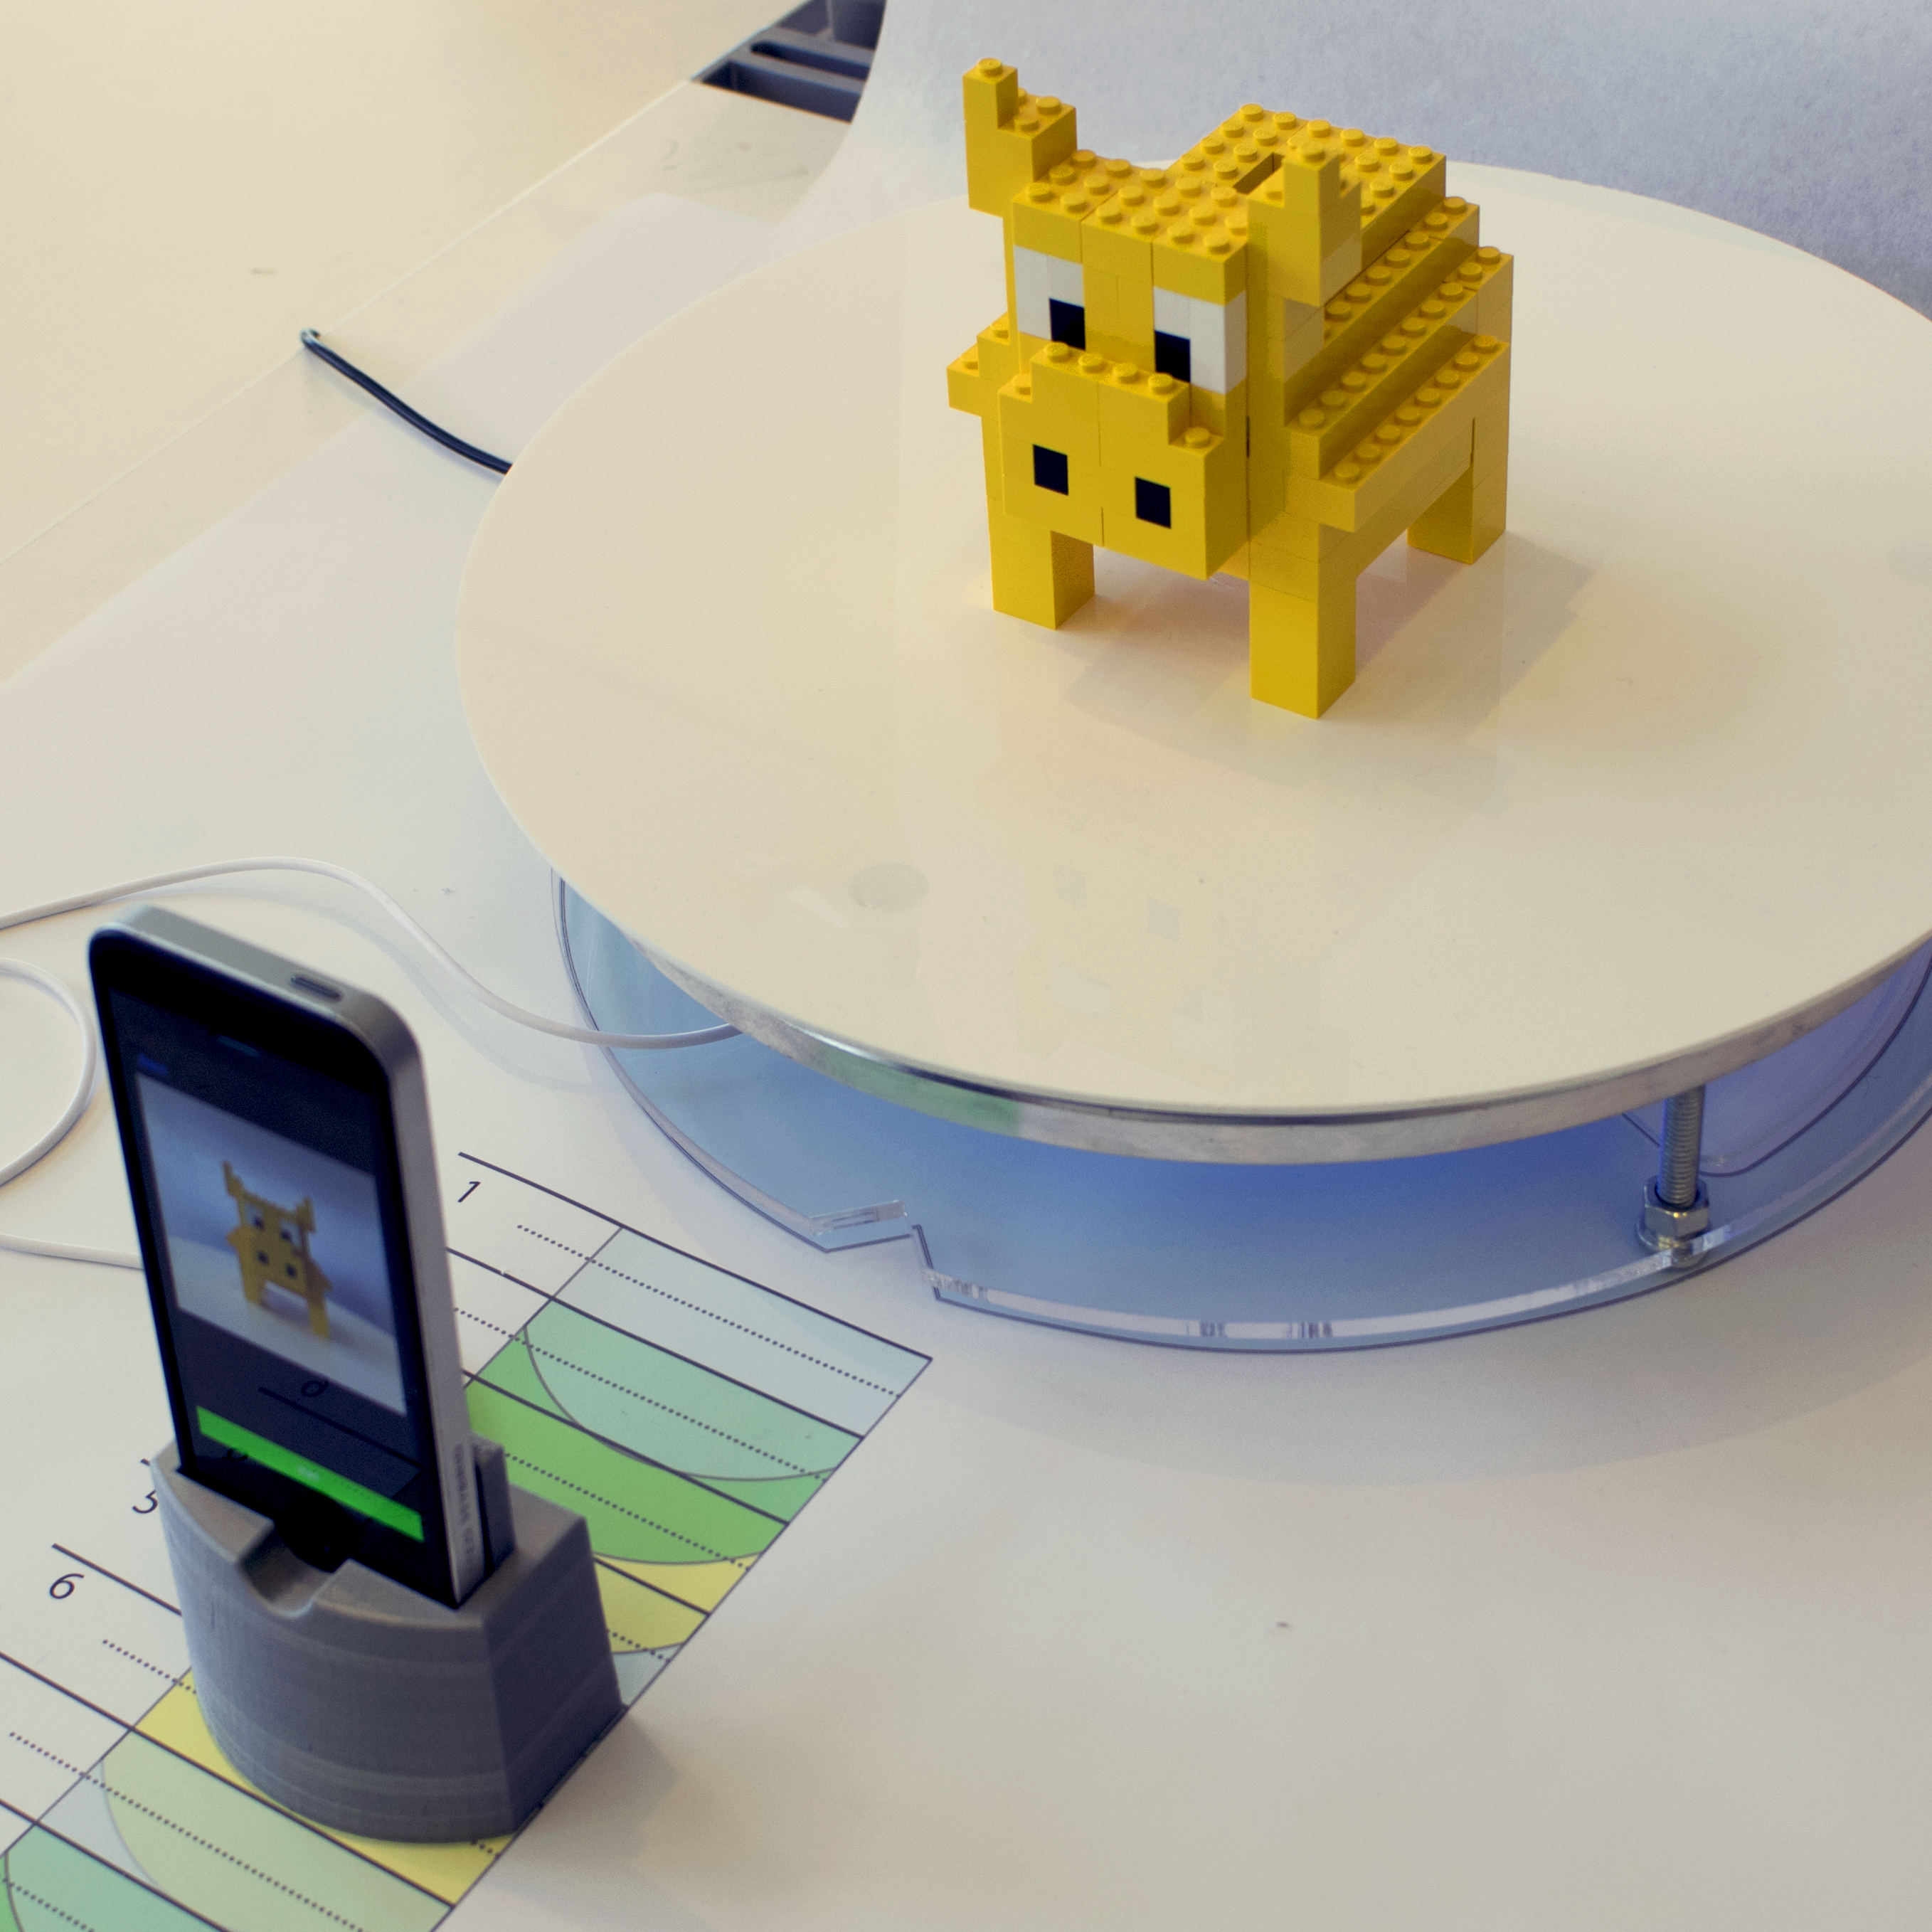
\includegraphics[width=\textwidth]{chap1/spin}               
% 	 \caption{Check it out, it's a Spin margin figure \url{spin.media.mit.edu}}
%  	\label{fig:spin_margin}
%\end{marginfigure}

%\begin{figure}[htb]
% 	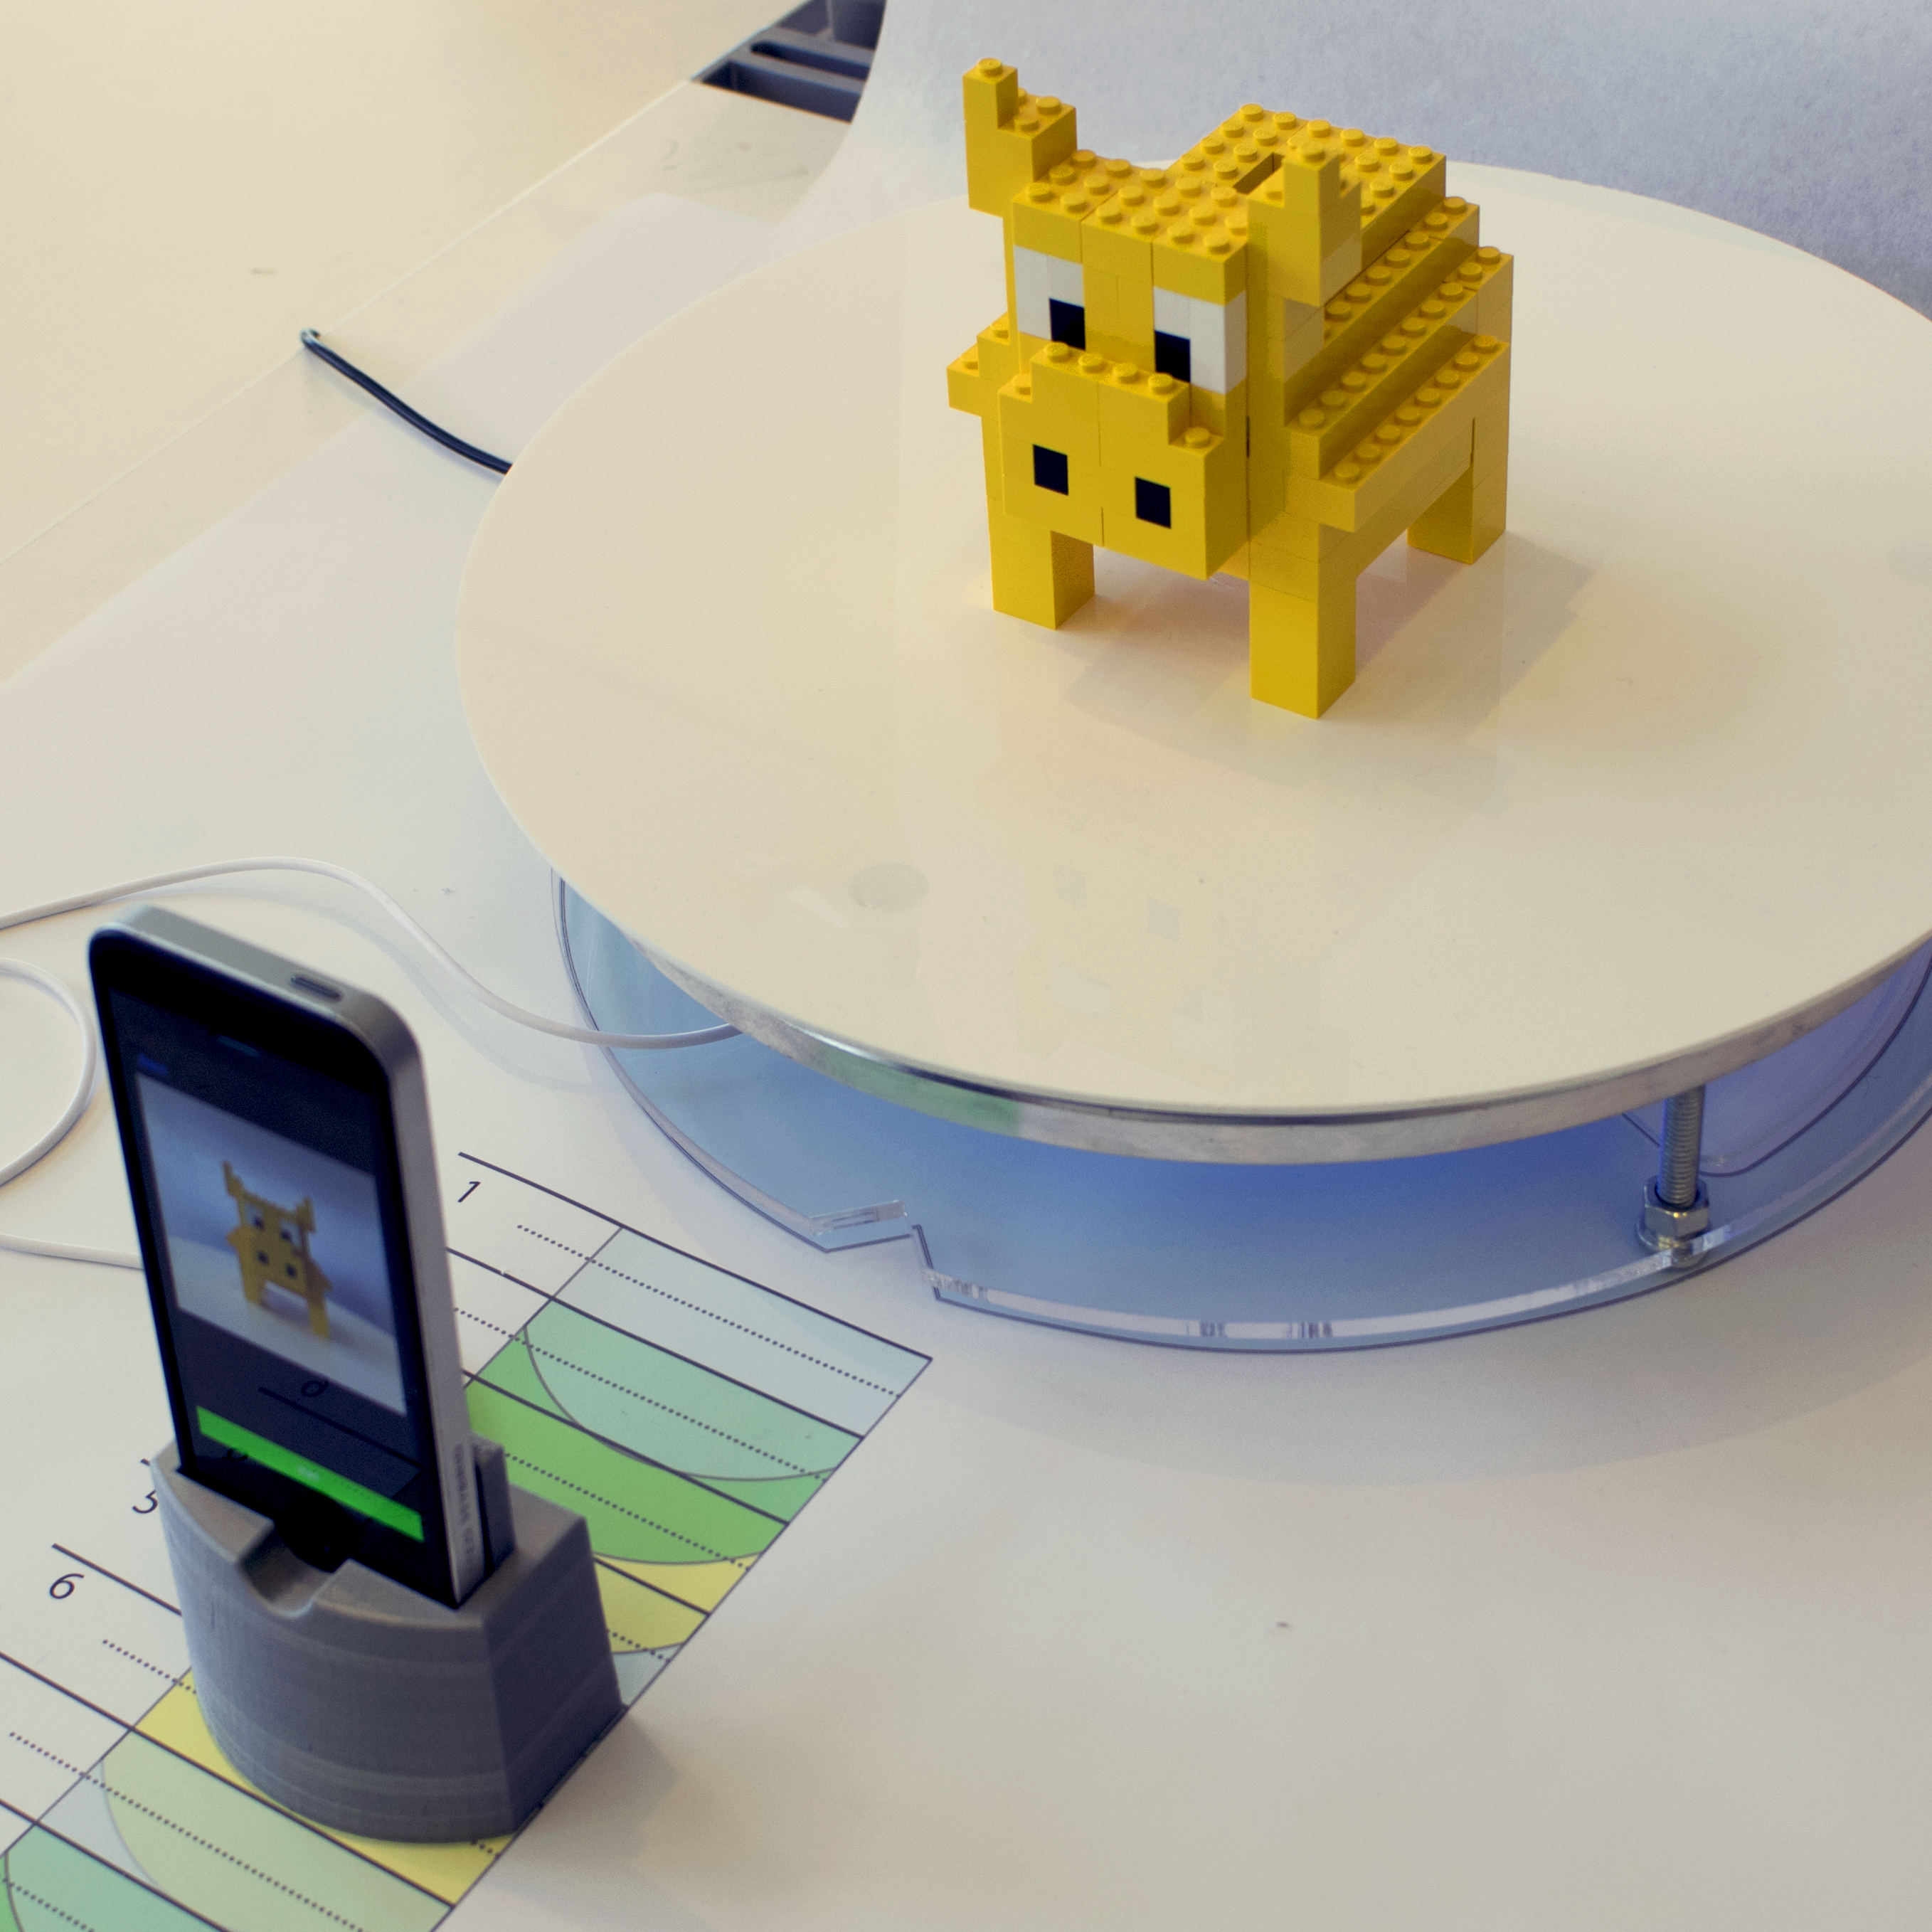
\includegraphics[width=\textwidth]{chap1/spin}               
% 	 \caption{Check it out, it's a Spin \url{spin.media.mit.edu}}
%  	\label{fig:spin}
%\end{figure}
